%% abtex2-modelo-trabalho-academico.tex, v-1.9.7 laurocesar
%% Copyright 2012-2018 by abnTeX2 group at http://www.abntex.net.br/ 
%%
%% This work may be distributed and/or modified under the
%% conditions of the LaTeX Project Public License, either version 1.3
%% of this license or (at your option) any later version.
%% The latest version of this license is in
%%   http://www.latex-project.org/lppl.txt
%% and version 1.3 or later is part of all distributions of LaTeX
%% version 2005/12/01 or later.
%%
%% This work has the LPPL maintenance status `maintained'.
%% 
%% The Current Maintainer of this work is the abnTeX2 team, led
%% by Lauro César Araujo. Further information are available on 
%% http://www.abntex.net.br/
%%
%% This work consists of the files abntex2-modelo-trabalho-academico.tex,
%% abntex2-modelo-include-comandos and abntex2-modelo-references.bib
%%

% ------------------------------------------------------------------------
% ------------------------------------------------------------------------
% abnTeX2: Modelo de Trabalho Academico (tese de doutorado, dissertacao de
% mestrado e trabalhos monograficos em geral) em conformidade com 
% ABNT NBR 14724:2011: Informacao e documentacao - Trabalhos academicos -
% Apresentacao
% ------------------------------------------------------------------------
% ------------------------------------------------------------------------

\documentclass[
	% -- opções da classe memoir --
	12pt,				 % tamanho da fonte
	oneside,			 % para impressão em recto.
	a4paper,			 % tamanho do papel.
	% -- opções da classe abntex2 --
	chapter=TITLE,		 % títulos de capítulos convertidos em letras maiúsculas
	section=TITLE,		 % títulos de seções convertidos em letras maiúsculas
	sumario=tradicional, % estilo do sumário (tradicional = indentado)
	% -- opções do pacote babel --
	english,			 % idioma adicional para hifenização
	french,				 % idioma adicional para hifenização
	spanish,			 % idioma adicional para hifenização
	brazil				 % o último idioma é o principal do documento
	]{abntex2}

% ---
% Pacotes básicos 
% ---
\usepackage{helvet}			    % Usa a fonte Helvet			
\usepackage[T1]{fontenc}		% Selecao de codigos de fonte.
\usepackage[utf8]{inputenc}		% Codificacao do documento (conversão automática dos acentos)
\usepackage{indentfirst}		% Indenta o primeiro parágrafo de cada seção.
\usepackage{color}				% Controle das cores
\usepackage{graphicx}			% Inclusão de gráficos
\usepackage{microtype} 			% Para melhorias de justificação
\usepackage{lib/unifacens}      % Adaptações as normas da UniFacens
\usepackage{pdfpages}           % Para incluir pdf no documento
\usepackage{ragged2e}           % Para alinhamento de texto
\usepackage{titlesec}
\usepackage{booktabs} % adiciona italico
% ---
		
% ---
% Pacotes adicionais, usados apenas no âmbito do Modelo Canônico do abnteX2
% ---
\usepackage{lipsum}				% para geração de dummy text
% ---

% ---
% Pacotes de citações
% ---
\usepackage[brazilian,hyperpageref]{backref}	 % Paginas com as citações na bibl
\usepackage[alf]{abntex2cite}	% Citações padrão ABNT


% --- 
% CONFIGURAÇÕES DE PACOTES
% --- 

% ---
% Configurações do pacote backref
% Usado sem a opção hyperpageref de backref
\renewcommand{\backrefpagesname}{Citado na(s) página(s):~}
% Texto padrão antes do número das páginas
\renewcommand{\backref}{}
% Define os textos da citação
\renewcommand*{\backrefalt}[4]{
	\ifcase #1 %
		Nenhuma citação no texto.%
	\or
		Citado na página #2.%
	\else
		Citado #1 vezes nas páginas #2.%
	\fi}%
% ---

% --- 
% CONFIGURAÇÕES DE ESTILO E TAMANHO DA FONTE
% --- 

% Define a fonte padrão como serif (Arial)
\renewcommand{\familydefault}{\sfdefault}

% Define o tamanho da fonte dos capitulos para 14pt.
\renewcommand*{\chapnumfont}{\normalfont\large\bfseries\sffamily}
\renewcommand*{\chaptitlefont}{\normalfont\large\bfseries\sffamily}

% Define o tamanho da fonte das seções e sub-seções para 12pt,
% sendo as seções em negrito.
\setsecheadstyle{\normalsize\bfseries}
\setsubsecheadstyle{\normalsize}
% ---

\graphicspath{{./images/}}

% ---
% Informações sobre o trabalho
% ---
\coordenadoria{Coordenadoria de Engenharia da Computação}
\titulo{Plataforma de Freelance em Blockchain}
% \subtitulo{Subtitulo se houver}
\integranteum{Vinícius Lourenço Claro Cardoso}
\integrantedois{Henrique Rodrigues Silva}
\local{Sorocaba/SP}
\data{2022}

% ---
% Informações sobre orientador
% ---
\orientador{Kleber de Jesus Dias}

% ---
% Informações sobre coorientador
% ---
\coorientador{}

% O preambulo deve conter o tipo do trabalho, o objetivo, 
% o nome da instituição e a área de concentração 
\preambulo{Trabalho de conclusão de curso apresentado ao Centro Universitário Facens como exigência parcial para obtenção do diploma de graduação em Engenharia da Computação.\\ Orientador: Prof. Kleber de Jesus Dias}
% ---


% ---
% Configurações de aparência do PDF final

% alterando o aspecto da cor azul
\definecolor{blue}{RGB}{41,5,195}

% informações do PDF
\makeatletter
\hypersetup{
     	%pagebackref=true,
		pdftitle={\@title}, 
		pdfauthor={\@author},
    	pdfsubject={\imprimirpreambulo},
	    pdfcreator={LaTeX with abnTeX2},
		pdfkeywords={abnt}{latex}{abntex}{abntex2}{trabalho acadêmico}, 
		colorlinks=true,       		% false: boxed links; true: colored links
    	linkcolor=black,          	% color of internal links
    	citecolor=blue,        		% color of links to bibliography
    	filecolor=magenta,      		% color of file links
		urlcolor=blue,
		bookmarksdepth=4
}
\makeatother
% --- 

% ---
% Posiciona figuras e tabelas no topo da página quando adicionadas sozinhas
% em um página em branco. Ver https://github.com/abntex/abntex2/issues/170
\makeatletter
\setlength{\@fptop}{5pt} % Set distance from top of page to first float
\makeatother
% ---

% ---
% Possibilita criação de Quadros e Lista de quadros.
% Ver https://github.com/abntex/abntex2/issues/176
%
\newcommand{\quadroname}{Quadro}
\newcommand{\listofquadrosname}{Lista de quadros}

\newfloat[chapter]{quadro}{loq}{\quadroname}
\newlistof{listofquadros}{loq}{\listofquadrosname}
\newlistentry{quadro}{loq}{0}

% configurações para atender às regras da ABNT
\setfloatadjustment{quadro}{\centering}
\counterwithout{quadro}{chapter}
\renewcommand{\cftquadroname}{\quadroname\space} 
\renewcommand*{\cftquadroaftersnum}{\hfill--\hfill}

\setfloatlocations{quadro}{hbtp} % Ver https://github.com/abntex/abntex2/issues/176
% ---

% --- 
% Espaçamentos entre linhas e parágrafos 
% --- 

% O tamanho do parágrafo é dado por:
\setlength{\parindent}{1.3cm}

% Controle do espaçamento entre um parágrafo e outro:
\setlength{\parskip}{0.2cm}  % tente também \onelineskip

% Controle do espaçamento após um capitulo, seção e sub-seção
\setlength{\afterchapskip}{\baselineskip}
\setlength{\aftersecskip}{\baselineskip}
\setlength{\aftersubsecskip}{\baselineskip}

% ---
% compila o indice
% ---
\makeindex
% ---

% ----
% Início do documento
% ----
\begin{document}

% Seleciona o idioma do documento (conforme pacotes do babel)
%\selectlanguage{english}
\selectlanguage{brazil}

% Retira espaço extra obsoleto entre as frases.
\frenchspacing 

% ----------------------------------------------------------
% ELEMENTOS PRÉ-TEXTUAIS
% ----------------------------------------------------------
\imprimircapa
\imprimirfolhaderosto*

% TODO: Adicionar de volta quando obter a ficha \begin{fichacatalografica}
	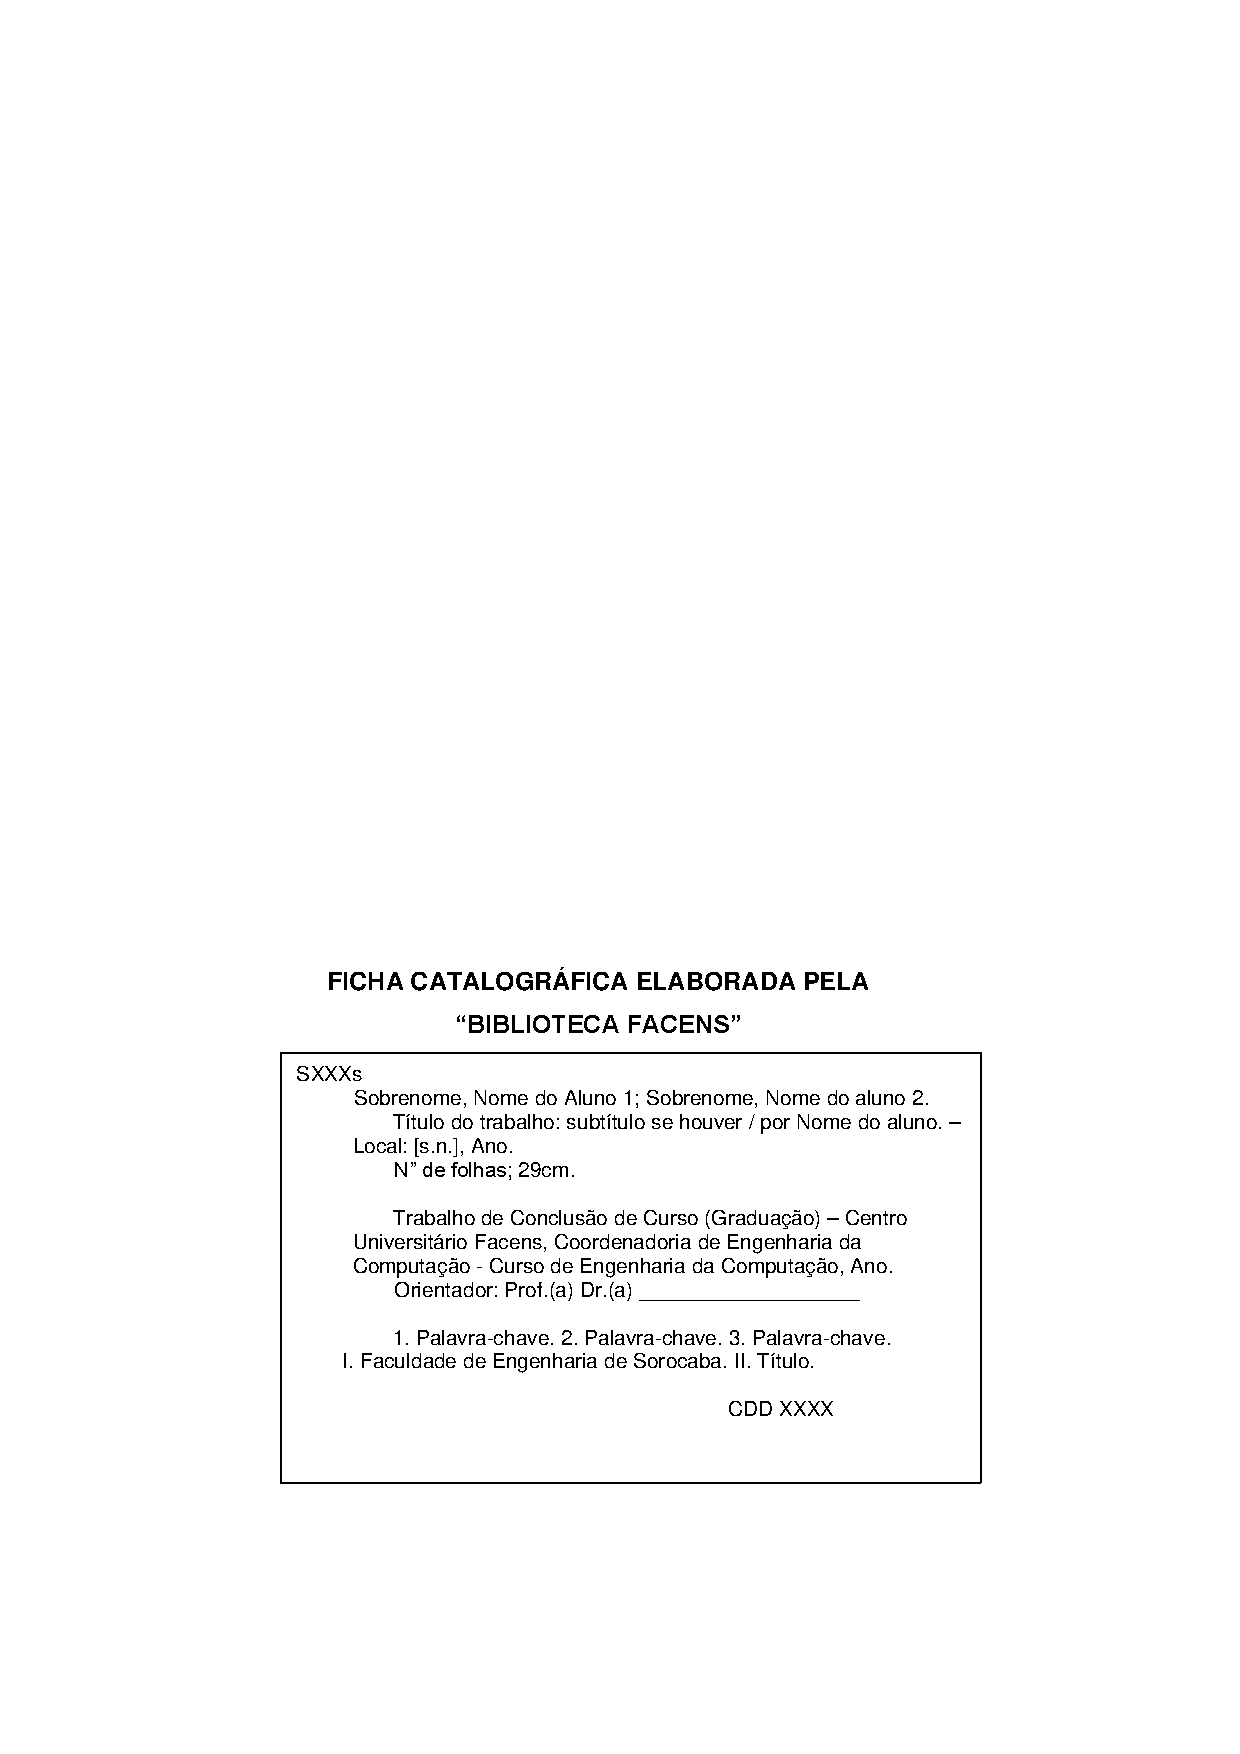
\includepdf[page=1]{partes/pre_textuais/ficha_catalografica.pdf}
\end{fichacatalografica}
% TODO: Adicionar de volta quando obter a folha de aprovação \begin{folhadeaprovacao}
	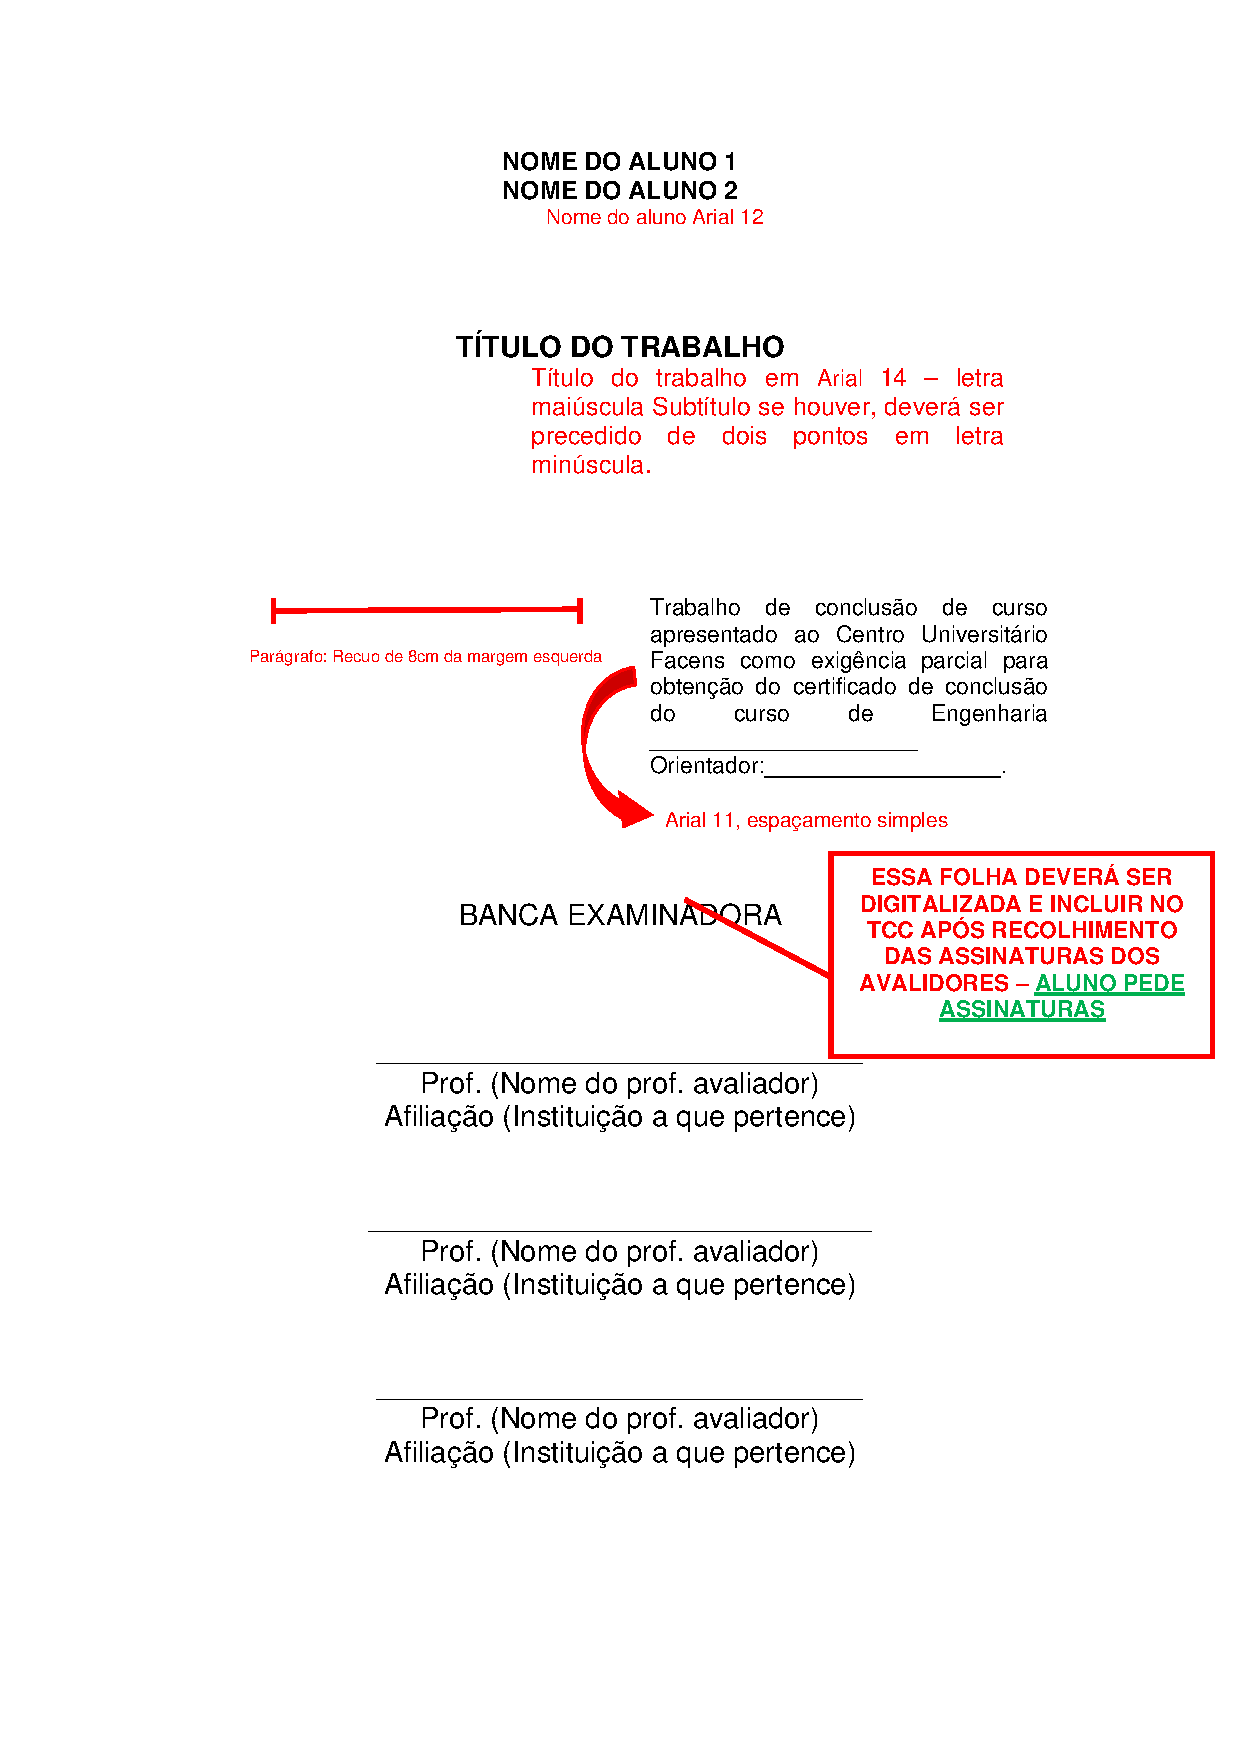
\includepdf[page=1]{partes/pre_textuais/folha_aprovacao.pdf}
\end{folhadeaprovacao}
% TODO: Adicioanr de volta quando começar a escrever os agradecimentos \begin{agradecimentos}
    Os agradecimentos principais são direcionados à Gerald Weber, Miguel Frasson,
    Leslie H. Watter, Bruno Parente Lima, Flávio de Vasconcellos Corrêa, Otavio Real
    Salvador, Renato Machnievscz e todos aqueles que
    contribuíram para que a produção de trabalhos acadêmicos conforme
    as normas ABNT com \LaTeX\ fosse possível.

    Agradecimentos especiais são direcionados ao Centro de Pesquisa em Arquitetura
    da Informação da Universidade de
    Brasília (CPAI), ao grupo de usuários
    \emph{latex-br} e aos
    novos voluntários do grupo
    \emph{\abnTeX} e que contribuíram e que ainda
    contribuirão para a evolução do \abnTeX.
\end{agradecimentos}
% TODO: Adicionar de volta quando entender para que serve \begin{epigrafe}
    \vspace*{\fill}
    
    \begin{flushright}
        \begin{minipage}{8cm}
            \begin{SingleSpace}
                ``Não vos amoldeis às estruturas deste mundo,
                mas transformai-vos pela renovação da mente,
                a fim de distinguir qual é a vontade de Deus:
                o que é bom, o que Lhe é agradável, o que é perfeito.``\\
                (Bíblia Sagrada, Romanos 12, 2)
            \end{SingleSpace}
        \end{minipage}
    \end{flushright}
\end{epigrafe}
% TODO: Adicionar de volta quando for escrever o resumo % resumo em português
\setlength{\absparsep}{18pt} % ajusta o espaçamento dos parágrafos do resumo
\begin{resumo}
    Segundo a \citeonline[3.1-3.2]{NBR6028:2003}, o resumo deve ressaltar o
    objetivo, o método, os resultados e as conclusões do documento. A ordem e a extensão
    destes itens dependem do tipo de resumo (informativo ou indicativo) e do
    tratamento que cada item recebe no documento original. O resumo deve ser
    precedido da referência do documento, com exceção do resumo inserido no
    próprio documento. (\ldots) As palavras-chave devem figurar logo abaixo do
    resumo, antecedidas da expressão Palavras-chave:, separadas entre si por
    ponto e finalizadas também por ponto.

    \textbf{Palavras-chave}: latex. abntex. editoração de texto.
\end{resumo}

% resumo em inglês
\begin{resumo}[Abstract]
    \begin{otherlanguage*}{english}
        This is the ddd abstract.

        \vspace{\onelineskip}

        \noindent 
        \textbf{Keywords}: latex. abntex. text editoration.
    \end{otherlanguage*}
\end{resumo}
% TODO: Adicionar de volta quando tiver alguma figura \pdfbookmark[0]{\listfigurename}{lof}
\listoffigures*
\cleardoublepage
% TODO: Adicionar de volta quando tiver algum quadro \pdfbookmark[0]{\listofquadrosname}{loq}
\listofquadros*
\cleardoublepage
% TODO: Adicionar de volta quando tiver alguma tabela \pdfbookmark[0]{\listtablename}{lot}
\listoftables*
\cleardoublepage
\begin{siglas}
    \item[IPFS] InterPlanetary File System - Sistema de Arquivos Interplanetário.
    \item[Freelancer] É um termo para descrever o profissional autónomo que realiza serviços para outras empresas.
    \item[Workana] É uma empresa que fornece uma plataforma de Freelance.
    \item[Upwork] Assim como o Workana, é empresa que fornece uma plataforma de Freelance.
\end{siglas}
\pdfbookmark[0]{\contentsname}{toc}
\tableofcontents*
\cleardoublepage

% ----------------------------------------------------------
% ELEMENTOS TEXTUAIS
% ----------------------------------------------------------
\chapter{Introdução}
% ----------------------------------------------------------

Em 2008, Satoshi Nakamoto descreveu em um trabalho que foi chamado de \textit{Bitcoin: A Peer-to-Peer Eletronic Cash System} uma maneira de realizar pagamentos digitais, ao utilizar criptomoedas, de forma descentralizada. Isso significa que para realizar a transferência de um valor para outra pessoa, não é necessário que uma instituição financeira para validar que quem está transferindo realmente possui o valor, a própria rede do \textit{Bitcoin} garantirá essa validação, resolvendo assim o problema do gasto-duplo.\cite{bitcoin}

A tecnologia principal que move esse sistema de pagamento é o \textit{Blockchain}, uma maneira de armazenar dados de forma extremamente segura que funciona como uma lista de blocos que são interligados uns aos outros de forma a garantir que os dados registrados nos blocos sejam imutáveis.\cite{blockchain}

A partir dessa tecnologia, em 2014, Vitalik Buterin publicou um trabalho para apresentar o \textit{Ethereum}, um protocolo que roda com a tecnologia de Blockchain e permite criar aplicações decentralizadas através de \textit{Smart Contracts}.\cite{ethereum} \cite{ethereum_yellow} Os \textit{Smart Contracts} é uma forma de escreve um contrato que pode ser executado de forma automática.\cite{smart_contract} \cite{smart_contract_blockchain}

Com essas tecnologias, em 2022, é possível realizar pagamentos entre pessoas de qualquer parte do mundo sem que ninguém possa impedir, e também ter a posse digital de uma obra de arte onde você tem uma prova imutável de que você é o dono dela. Em um mundo onde tudo está cada vez mais conectado, a necessidade de ter sistemas distribuídos está se mostrando uma peça fundamental para a liberdade individual, de forma que, você possa comprar ou ter algo sem que ninguém possa censurar ou retirar de você.\cite{decentralization}

Contudo, ainda é necessário que você possua dinheiro no mundo digital para que você possa realizar pagamentos e compras, e uma das formas de ganhar dinheiro é através de \textit{Freelance}, onde você realiza algum trabalho e recebe por esse trabalho. Ao pensar sobre as soluções existentes hoje, temos o Workana e Upwork mas são plataformas que tem toda a sua estrutura centralizada e não realizam pagamentos em criptomoeda.

Com isso, o problema que esse trabalho se propõe a resolver é a criação de uma plataforma de \textit{Freelance} totalmente descentralizada, de forma que, você possa postar projetos e ser contratado para um projeto recebendo por esse trabalho em criptomoeda. Além disso, com um sistema de resolução de conflitos e outro para pontuação, a ideia é incentivar bons \textit{Freelancers} a entrarem e continuarem na plataforma.

Essa plataforma tem como o objetivo de ser simples de ser usada, totalmente descentralizada com sistema de pontuação para premiar e evidenciar bons \textit{Freelancers}. Além disso, ao ser totalmente descentralizado, ela se diferenciará de outras plataformas de \textit{Freelance} em \textit{Blockchain} que possuem alguns dos seus sistemas centralizados em troca de melhorar a usabilidade.

Um ponto importante de uma plataforma de \textit{Freelance} é a resolução de conflitos e quando será feito os pagamentos, visto que, é possível que haja pessoas má intencionadas querendo roubar o dinheiro de um contratante, ou mesmo, o contratante não querendo pagar o \textit{Freelance}, esses dois problemas serão descritos nos próximos capítulos.

Para construir a plataforma, será utilizado principalmente \textit{Smart Contracts}, que rodará em uma rede de \textit{Blockchain} chamada \textit{Polygon}, uma alternativa para a \textit{Ethereum} que possui taxas de transações muito mais baixas, além de processar as transações mais rapidamente. E assim como na \textit{Ethereum}, que possui a moeda principal \textit{ether}, na \textit{Polygon} temos o Matic, que será usado para realizar o pagamento das taxas das transações.\cite{polygon}

Além dos \textit{Smart Contracts}, será criado um site que posteriormente será disponibilizado aos usuários através do protocolo \textit{IPFS}, que é um sistema de armazenamento permanente de arquivos de forma descentralizada. Uma vez que os arquivos estejam no sistema do \textit{IPFS}, para ser excluído, todos na rede que possuem uma cópia precisam ativamente excluir essa cópia.\cite{ipfs}

Para esse trabalho, é esperado no final dele a criação dos contratos inteligentes, assim como, um site para servir de interface para os contratos que estarão disponibilizados em uma rede de \textit{Blockchain} e no protocolo \textit{IPFS}. Contudo, esse trabalho não irá abranger a comunicação entre duas pessoas de forma descentralizada e anônima, a comunicação ainda será responsabilidade do contratante e do \textit{Freelancer}.

Este trabalho está organizado da seguinte maneira: no Capítulo 2 é será feito uma revisão teórica sobre os conceitos apresentados nessa introdução para explicar sobre a descentralização e como é feita a segurança de todo o sistema. No Capítulo 3 será apresentado as tecnologias e serviços utilizados para a criação da plataforma. No Capítulo 4 será mostrado detalhes da implementação da plataforma, além de mostrar o design dos \textit{Smart Contracts} e da estrutura do site construido assim como também será descrito as dificuldades e limitações de um sistema descentralizado. Por fim, nos Capítulos 5 será apresentado os conceitos, e no Capítulo 6, as conclusões assim como sugestões para trabalhos futuros.\cite{curses_of_blockchain}

% TODO: Adicionar de volta quando chegar na parte de escrever o referencial teórico \include{abntex2-modelo-include-comandos}

\chapter{Referencial teórico}\label{cap_trabalho_academico}

\section{Aliquam vestibulum fringilla lorem}

\lipsum[1]

\subsection{Pellentesque sit amet pede ac sem eleifend consectetuer}
\lipsum[2-3]
% TODO: Adicionar de volta quando chegar na parte de escrever o metodologias \chapter{Desenvolvimento}

\section{Quadros}

Este modelo vem com o ambiente \texttt{quadro} e impressão de Lista de quadros 
configurados por padrão. Verifique um exemplo de utilização:

\begin{quadro}[htb]
    \caption{\label{quadro_exemplo}Exemplo de quadro}
    \begin{tabular}{|c|c|c|c|}
        \hline
        \textbf{Pessoa} & \textbf{Idade} & \textbf{Peso} & \textbf{Altura} \\ \hline
        Marcos & 26    & 68   & 178    \\ \hline
        Ivone  & 22    & 57   & 162    \\ \hline
        ...    & ...   & ...  & ...    \\ \hline
        Sueli  & 40    & 65   & 153    \\ \hline
    \end{tabular}
    \fonte{Autor.}
\end{quadro}

Este parágrafo apresenta como referenciar o quadro no texto, requisito
obrigatório da ABNT. 
Primeira opção, utilizando \texttt{autoref}: Ver o \autoref{quadro_exemplo}. 
Segunda opção, utilizando  \texttt{ref}: Ver o Quadro \ref{quadro_exemplo}.
% TODO: Adicionar de volta quando chegar na parte de escrever o resultado % ---
% primeiro capitulo de Resultados
% ---
\chapter{Resultados}
% ---

% ---
\section{Vestibulum ante ipsum primis in faucibus orci luctus et ultrices
posuere cubilia Curae}
% ---

\lipsum[21-22]
% TODO: Adicionar de volta quando chegar na parte de escrever a conclusão \chapter{Conclusões}
% ---

\lipsum[31-33]

% ----------------------------------------------------------
% ELEMENTOS PÓS-TEXTUAIS
% ----------------------------------------------------------

\bibliography{abntex2-modelo-references}

Os textos abaixo serão removidos na versão final, eles estão aqui apenas como parte da entrega do Report 2.

\cite{bitcoin} 
A popularização do Blockchain começou quando o Bitcoin foi lançado, e muito dos conceitos de criptomoedas vem desse white-paper, por isso colocamos essa referência.

\cite{blockchain}
Com o white-paper do Bitcoin dando uma introdução sobre o conceito do Blockchain, nesse paper do MIT, eles definem o que é realmente o Blockchain e entram em tópicos mais avançados, e essa referência será usada para definir o termo Blockchain, assim como, falar dos detalhes de implementação ao mencionar outras redes de Blockchain.

\cite{ethereum}
É um white-paper do co-fundador do Ethereum que é uma das redes de Blockchain mais famosas e nela que este trabalho toma forma, apesar da implementação final não usar a Ethereum por conta de custos, é necessário falar e descrever o que é o Ethereum e a sua influência, assim como, entender os conceitos apresentados.

\cite{ethereum_yellow}
É um yellow-paper do co-fundador do Ethereum, Gavin Wood, e nesse yellow-paper temos uma descrição mais detalhada de como funciona o sistema que roda os Smart Contracts, e essas definições serão usadas para embasar os detalhes técnicos deste trabalho.

\cite{smart_contract}
É um paper de Nick Szabo, onde ele descreve uma das primeiras definições de Smart Contracts e esse trabalho é a referencia principal quando se trata de descrever o que são os Smart Contracts em sua natureza.

\cite{smart_contract_blockchain}
Nessa referencia, é uma continuação que aprofunda as explicações e definições de Smart Contracts definidas por Nick Szabo ao apresentar até mesmo a implementação de Smart Contracts em Solidity, assim como, fala também da aplicação de Smart Contracts para substituir contratos legais.

\cite{ipfs}
É o white-paper que descreve o que é o IPFS, o protocolo para salvar arquivos de forma permanente que será usado durante o contrato para hospedar o site.

\cite{decentralization}
Durante a criação do referencia teórico, esse trabalho de Markus Boeckenfoerde é uma peça importante para entender a motivação por trás do nosso trabalho de criar uma plataforma totalmente descentralizada de freelance, Markus em seu trabalho descreve como a descentralização ajuda a manter a paz e segurança em relações de governança entre entidades e indivíduos.

\cite{polygon}
Como mencionado anteriormente, não iremos usar a Ethereum, em vez disso, foi escolhido a rede Polygon que é mais nova que a Ethereum e possui custos de transação menores, e nesse white-paper, é definido o que é o Polygon e o Matic (a moeda da rede).

\cite{curses_of_blockchain}
Esse trabalho de Shumo Chu e Sophia Wang será usado para embasar melhor o motivo da escolha da implementação usando Polygon em vez do Ethereum, e também falar mais sobre os problemas que ocorrem ao criar uma solução totalmente descentralizada.

% TODO: Adicionar de volta se fizer sentido \begin{apendicesenv}
    \chapter{Quisque libero justo}
    \lipsum[50]

    \chapter{Nullam elementum urna vel imperdiet sodales elit ipsum pharetra ligula
    ac pretium ante justo a nulla curabitur tristique arcu eu metus}
    \lipsum[55-57]
\end{apendicesenv}
% TODO: Adicionar de volta se fizer sentido \begin{anexosenv}
    % coloca o primeiro anexo na mesma pagina do titulo do capitulo
    \chapter{Morbi ultrices rutrum lorem}
    \lipsum[30]

    \chapter{Cras non urna sed feugiat cum sociis natoque penatibus et magnis dis
    parturient montes nascetur ridiculus mus}
    \lipsum[31]

    \chapter{Fusce facilisis lacinia dui}
    \lipsum[32]
\end{anexosenv}

%---------------------------------------------------------------------
% INDICE REMISSIVO
%---------------------------------------------------------------------
\printindex
%---------------------------------------------------------------------

\end{document}
